\chapter{Évaluation et résultats}\label{chap:resultats}

Ce chapitre présente les performances du modèle sur le jeu de test (231 images jamais vues pendant l’entraînement ni le choix des hyperparamètres), analyse ses erreurs et décrit les expériences complémentaires qui ont guidé nos choix.

\section{Métriques d’évaluation}

Soit $TP_k$, $FP_k$ et $FN_k$ les vrais positifs, faux positifs et faux négatifs de la classe $k$. On définit~:
\begin{align}
  \text{exactitude} &= \frac{\text{prédictions correctes}}{\text{nombre total d’images}}, \\
  \text{précision}_k &= \frac{TP_k}{TP_k+FP_k}, \qquad
  \text{rappel}_k = \frac{TP_k}{TP_k+FN_k}, \\
  F1_k &= \frac{2\cdot \text{précision}_k\cdot\text{rappel}_k}{\text{précision}_k+\text{rappel}_k}.
\end{align}
La \textbf{précision} d’une classe répond à «~quand le modèle annonce cette classe, a-t-il raison~?~» et le \textbf{rappel} à «~parmi les vraies images de cette classe, combien sont retrouvées~?~». Le score F1 est leur moyenne harmonique. La \textbf{moyenne macro} calcule la moyenne simple de ces valeurs sur les 11 classes, sans tenir compte des effectifs~: elle est donc sensible aux classes rares, contrairement à l’exactitude.

\section{Résultats globaux}

Sur les 231 images de test, le modèle classe correctement 215, soit une \textbf{exactitude de 93,1\,\%}. Les moyennes macro sont une précision de 0,910, un rappel de 0,895 et un score F1 de 0,897. L’écart entre l’exactitude et la moyenne macro (environ trois points) reflète le fait que les classes rares sont un peu moins bien reconnues que les classes fréquentes.

\paragraph{Intervalle de confiance.} Avec 231 images de test, l’exactitude mesurée est elle-même incertaine. L’intervalle de Wilson à 95\,\% pour 215 réussites sur 231 essais est \textbf{[89,0\,\% ; 95,7\,\%]}. Il faut donc lire « environ 93\,\% » et non voir dans la décimale une garantie ; deux modèles dont les exactitudes diffèrent d’un ou deux points ne sont pas statistiquement distinguables sur ce test.

\section{Résultats par fruit}

\begin{table}[H]
\centering
\caption{Exactitude par fruit sur le jeu de test.}\label{tab:fruit}
\small
\begin{tabular}{@{}lrrr@{}}
\toprule
\textbf{Fruit} & \textbf{Images} & \textbf{Correctes} & \textbf{Exactitude} \\
\midrule
Banane & 101 & 99 & 98,0\,\% \\
Avocat & 87 & 81 & 93,1\,\% \\
Fraise & 43 & 35 & 81,4\,\% \\
\midrule
\textbf{Total} & \textbf{231} & \textbf{215} & \textbf{93,1\,\%} \\
\bottomrule
\end{tabular}
\end{table}

Les bananes sont presque parfaitement classées~: leurs trois stades ont des couleurs franches (vert, jaune, jaune tacheté de brun). Les fraises sont les plus difficiles~: c’est le fruit qui compte le moins d’images et dont les stades intermédiaires (rouge clair, rouge mûr) se ressemblent le plus.

\section{Résultats par classe}

\begin{table}[H]
\centering
\caption{Précision, rappel et F1 par classe sur le jeu de test.}\label{tab:classe}
\small
\begin{tabular}{@{}lrrrr@{}}
\toprule
\textbf{Classe} & \textbf{Précision} & \textbf{Rappel} & \textbf{F1} & \textbf{Support} \\
\midrule
Avocat mûr & 1,00 & 0,88 & 0,93 & 8 \\
Avocat non mûr & 0,95 & 0,83 & 0,88 & 23 \\
Avocat partiellement mûr & 0,80 & 0,94 & 0,86 & 17 \\
Avocat pourri & 0,97 & 1,00 & 0,99 & 39 \\
Banane mûre & 0,97 & 0,97 & 0,97 & 31 \\
Banane non mûre & 1,00 & 1,00 & 1,00 & 33 \\
Banane trop mûre & 0,97 & 0,97 & 0,97 & 37 \\
Fraise mûre & 0,63 & 0,91 & 0,74 & 11 \\
Fraise non mûre & 1,00 & 0,86 & 0,92 & 14 \\
Fraise partiellement mûre & 0,89 & 0,67 & 0,76 & 12 \\
Fraise pourrie & 0,83 & 0,83 & 0,83 & 6 \\
\midrule
\textbf{Moyenne macro} & \textbf{0,910} & \textbf{0,895} & \textbf{0,897} & 231 \\
\bottomrule
\end{tabular}
\end{table}

\begin{figure}[H]
\centering
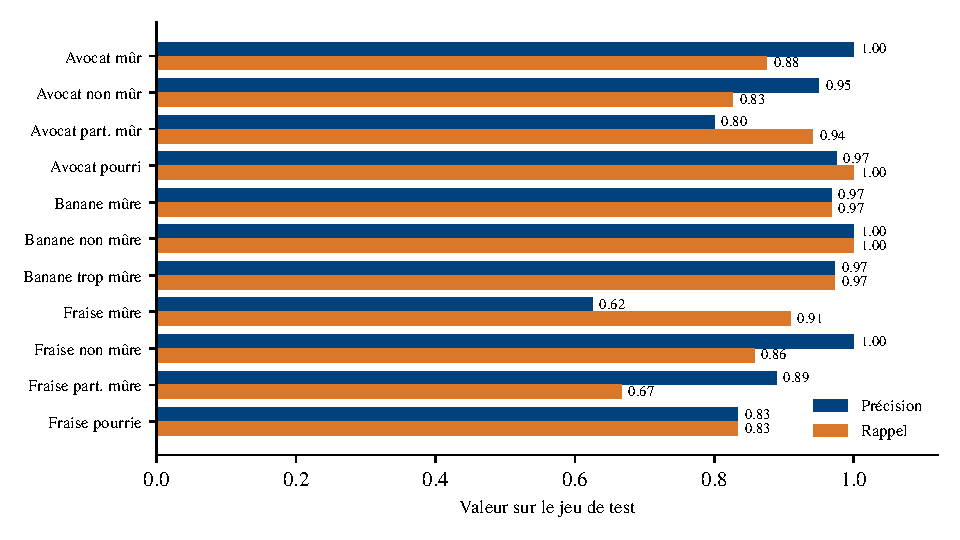
\includegraphics[width=0.95\textwidth]{figures/fig_prf.pdf}
\caption{Précision, rappel et F1 par classe.}\label{fig:prf}
\end{figure}

La «~fraise pourrie~» n’a que 6 images de test~: une seule erreur fait varier son rappel de 17 points. Les valeurs sur les classes de fraises et sur «~avocat mûr~» (8 images) doivent donc être interprétées avec prudence.

\section{Matrice de confusion}

La matrice de confusion (figure~\ref{fig:confusion}) compte, pour chaque classe réelle (lignes), les classes prédites (colonnes). La diagonale correspond aux bonnes réponses.

\begin{figure}[H]
\centering
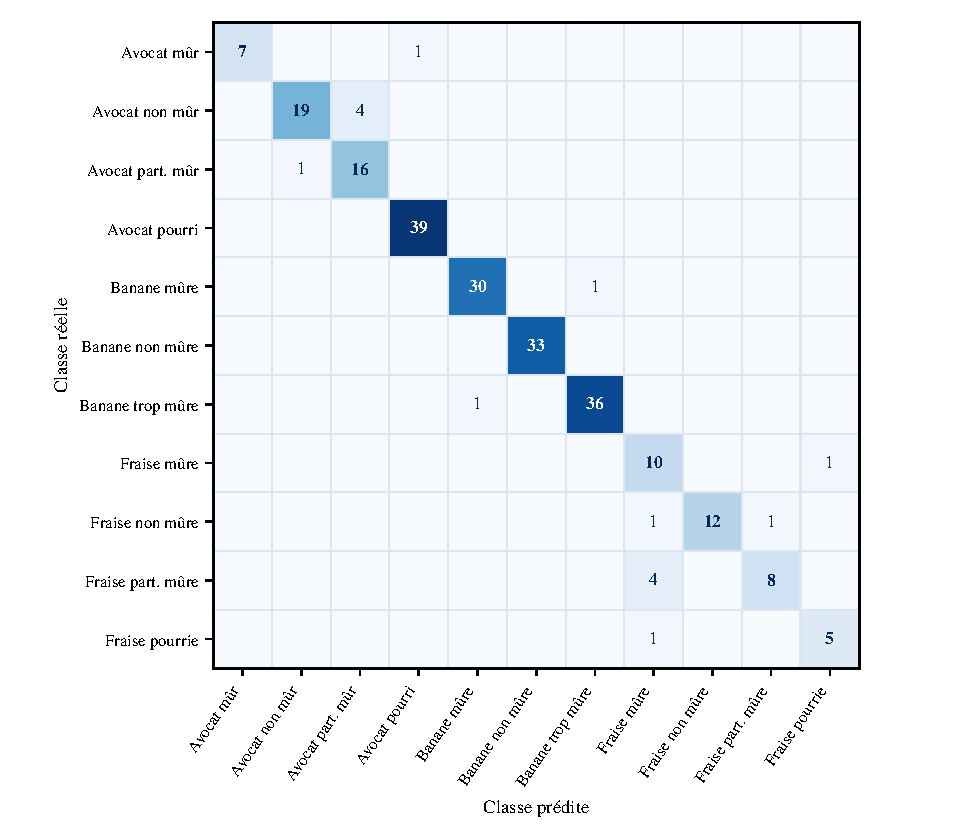
\includegraphics[width=0.92\textwidth]{figures/fig_confusion.pdf}
\caption{Matrice de confusion sur le jeu de test (231 images).}\label{fig:confusion}
\end{figure}

Le modèle commet \textbf{16 erreurs}. Elles sont toutes concentrées entre des stades \emph{voisins} du même fruit, ou entre «~mûr~» et «~pourri~»~:

\begin{table}[H]
\centering
\caption{Inventaire des 16 erreurs de classification.}\label{tab:erreurs}
\small
\begin{tabular}{@{}llr@{}}
\toprule
\textbf{Classe réelle} & \textbf{Classe prédite} & \textbf{Nombre} \\
\midrule
Avocat non mûr & Avocat partiellement mûr & 4 \\
Fraise partiellement mûre & Fraise mûre & 4 \\
Avocat mûr & Avocat pourri & 1 \\
Avocat partiellement mûr & Avocat non mûr & 1 \\
Banane mûre & Banane trop mûre & 1 \\
Banane trop mûre & Banane mûre & 1 \\
Fraise mûre & Fraise pourrie & 1 \\
Fraise non mûre & Fraise mûre & 1 \\
Fraise non mûre & Fraise partiellement mûre & 1 \\
Fraise pourrie & Fraise mûre & 1 \\
\midrule
\textbf{Total} & & \textbf{16} \\
\bottomrule
\end{tabular}
\end{table}

\paragraph{Analyse.} Aucune confusion ne mélange deux fruits différents~: l’identification du fruit est donc fiable à 100\,\% sur ce test. Toutes les erreurs portent sur le stade de maturité. Huit des seize erreurs relèvent de deux familles bien identifiées :

\begin{itemize}
  \item les \textbf{avocats non mûrs pris pour partiellement mûrs} (4 cas), et les \textbf{fraises partiellement mûres prises pour mûres} (4 cas). Dans les deux cas, le modèle choisit le stade voisin~: la maturité est un continuum et la frontière entre deux classes est floue, y compris pour un annotateur humain~;
  \item quelques erreurs isolées entre stades adjacents (banane mûre/trop mûre, fraise non mûre/mûre).
\end{itemize}

Ces erreurs sont de faible gravité pratique, puisque l’utilisateur n’est jamais induit en erreur sur le fruit et se trompe rarement de plus d’un cran de maturité. L’erreur la plus sérieuse est «~avocat mûr prédit pourri~» (1 cas), qui pourrait conduire à jeter un fruit consommable.

\section{Expériences complémentaires}

Pour évaluer la robustesse de nos choix, nous avons mené plusieurs variantes d’entraînement. Elles diffèrent par la configuration, mais pas par le jeu de test, sauf la dernière (tableau~\ref{tab:exp}).

\begin{table}[H]
\centering
\caption{Résumé des expériences et exactitudes sur le jeu de test.}\label{tab:exp}
\small
\begin{tabularx}{\textwidth}{@{}lXr@{}}
\toprule
\textbf{N°} & \textbf{Configuration} & \textbf{Exactitude} \\
\midrule
1 & Première version, callbacks réutilisés entre les deux phases & 90,0\,\% \\
2 & Callbacks recréés, BatchNorm gelées (\textbf{modèle retenu}) & \textbf{93,1\,\%} \\
3 & Augmentation renforcée (rotation 0,2, translation, bruit gaussien, dropout 0,4, 60 couches dégelées) & 90,9\,\% \\
4 & Ajout de 624 images de bananes d’une autre source (test de 352 images) & 86,6\,\% \\
\bottomrule
\end{tabularx}
\end{table}

\begin{figure}[H]
\centering
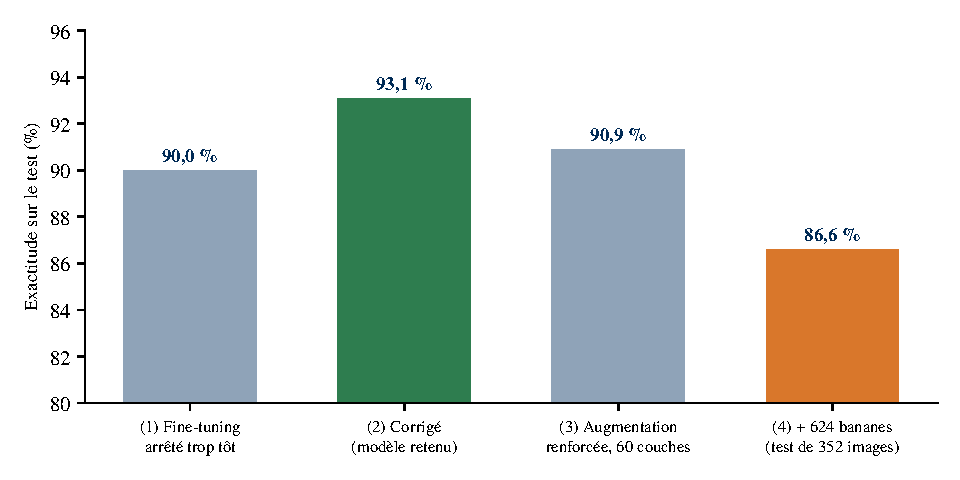
\includegraphics[width=0.78\textwidth]{figures/fig_experiences.pdf}
\caption{Exactitude de test des quatre expériences.}\label{fig:exp}
\end{figure}

\paragraph{Expérience 3~: augmenter plus fort n’aide pas.} Avec une augmentation plus agressive (retournement vertical, rotation jusqu’à 20\,\%, translation, bruit gaussien, dropout de 0,4) et 60 couches dégelées, l’exactitude tombe à 90,9\,\% (91,3\,\% après conversion TFLite). Avec 1\,118 images, des transformations trop fortes déforment les fruits au point de brouiller les indices utiles. La différence avec le modèle retenu (2,2 points) reste dans l’intervalle d’incertitude du test, mais aucune amélioration n’est observée ; nous conservons donc la configuration la plus simple.

\paragraph{Expérience 4~: plus de données, mais d’une autre origine.} Nous avons ajouté 624 images de bananes issues d’un jeu externe (collecte web, préfixe \code{web\_}), réparties en 432 images d’entraînement, 96 de validation et 96 de test, ce qui porte les ensembles à 1\,517, 353 et 352 images. L’exactitude globale baisse à 86,6\,\% : sur les 96 images \code{web\_}, elle n’est que de 80,2\,\%, contre 89,1\,\% sur le reste du test. Le rappel de « banane trop mûre » tombe à 0,68.

L’explication la plus plausible est une \textbf{incohérence d’étiquetage} entre les sources~: ce qu’un annotateur appelle «~trop mûre~» n’est pas ce qu’un autre appelle ainsi, et les bananes web ont des conditions de prise de vue différentes. C’est une leçon importante~: \emph{ajouter des données n’améliore le modèle que si elles sont étiquetées selon la même convention}. Nous n’avons pas retenu cette variante.

\section{Synthèse}

\begin{keybox}{Ce qu’il faut retenir}
\begin{itemize}[leftmargin=*,itemsep=2pt]
  \item Exactitude de test~: \textbf{93,1\,\%} (IC à 95\,\% : 89,0--95,7\,\%), F1 macro 0,897.
  \item Le fruit est toujours bien identifié~; les erreurs portent sur des stades voisins.
  \item Les bananes sont presque parfaites (98\,\%), les fraises les moins bien reconnues (81\,\%).
  \item Plus de données ou plus d’augmentation n’ont pas amélioré le modèle~: la qualité et la cohérence des étiquettes comptent plus que la quantité.
\end{itemize}
\end{keybox}
